%\documentclass[a4paper,12pt]{report}
\documentclass[a4paper,12pt]{article}
%\documentclass[a4paper,12pt]{book}
\usepackage{polski}
\usepackage[polish]{babel}
\usepackage[utf8]{inputenc}
\usepackage[top=2.5cm, bottom=2.5cm, left=3cm, right=2.5cm]{geometry}
\usepackage{graphicx}
\usepackage{setspace}
\usepackage{ifthen}
%\usepackage[utf8]{inputenc}
\usepackage{a4wide}
\usepackage{fullpage}
\usepackage{verbatim}
\usepackage[usenames,dvipsnames]{color}
\usepackage{hyperref}
\usepackage{subfig}
\usepackage{listings}
\usepackage{mdwlist}
\usepackage{titlesec}
\usepackage{lipsum}
\usepackage{morefloats}

\begin{document}

\begin{figure}[!htb]
\centering 		
  \subfloat[Windows]{
\includegraphics[width=0.45\textwidth]{images/aboutW}}    
  \hspace{2mm}
  \subfloat[Linux]{
\includegraphics[width=0.45\textwidth]{images/aboutL}}
\caption{Okno o programie} 	
\label{about}
\end{figure}

\begin{figure}[!htb]
\centering 		
  \subfloat[Windows]{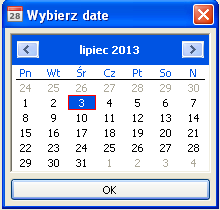
\includegraphics[width=0.25\textwidth]{images/calendarW}}    
  \hspace{2mm}
  \subfloat[Linux]{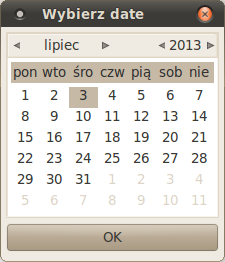
\includegraphics[width=0.25\textwidth]{images/calendarL}}
\caption{Okno wyboru daty} 	
\label{calendar}
\end{figure}

\begin{figure}[!htb]
\centering 		
  \subfloat[Windows]{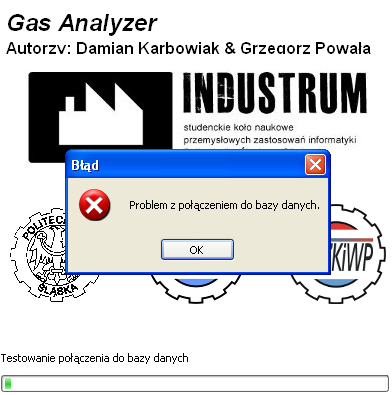
\includegraphics[width=0.35\textwidth]{images/dbErrorW}}    
  \hspace{2mm}
  \subfloat[Linux]{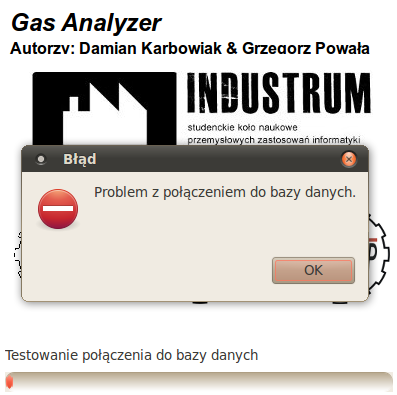
\includegraphics[width=0.35\textwidth]{images/dbErrorL}}
\caption{Komunikat o błędzie łączenia do bazy danych} 	
\label{dbError}
\end{figure}

\begin{figure}[!htb]
\centering 		
  \subfloat[Windows]{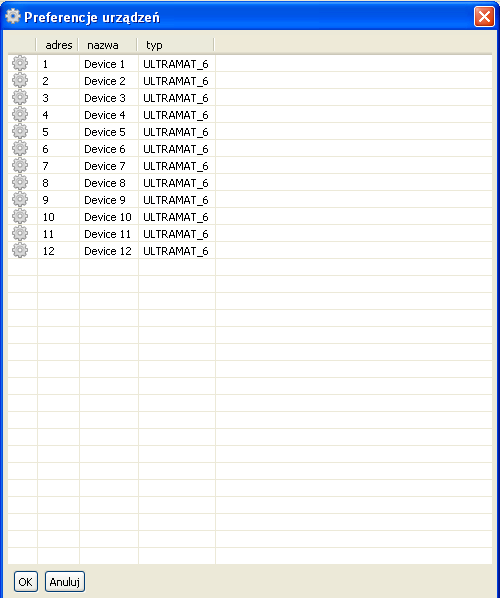
\includegraphics[width=0.45\textwidth]{images/editDeviceW}}    
  \hspace{2mm}
  \subfloat[Linux]{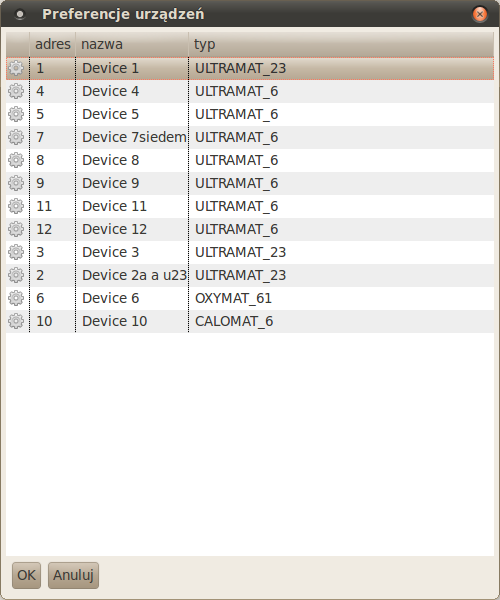
\includegraphics[width=0.45\textwidth]{images/editDeviceL}}
\caption{Okno edycji danych urzadzeń} 	
\label{editDevice}
\end{figure}

\begin{figure}[!htb]
\centering 		
  \subfloat[Windows]{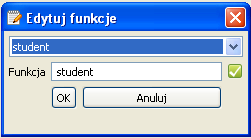
\includegraphics[width=0.45\textwidth]{images/editfFunctionW}}    
  \hspace{2mm}
  \subfloat[Linux]{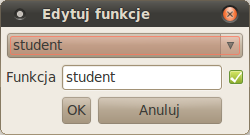
\includegraphics[width=0.45\textwidth]{images/editfFunctionL}}
\caption{Okno edycji funkcji} 	
\label{editFunction}
\end{figure}

\begin{figure}[!htb]
\centering 		
  \subfloat[Windows]{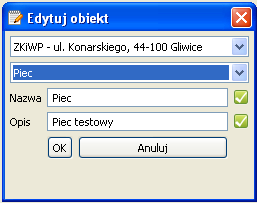
\includegraphics[width=0.45\textwidth]{images/editObjectW}}    
  \hspace{2mm}
  \subfloat[Linux]{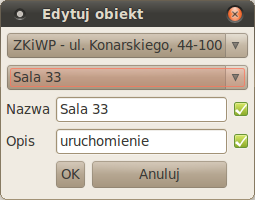
\includegraphics[width=0.45\textwidth]{images/editObjectL}}
\caption{Okno edycji obiektów} 	
\label{editObject}
\end{figure}

\begin{figure}[!htb]
\centering 		
  \subfloat[Windows]{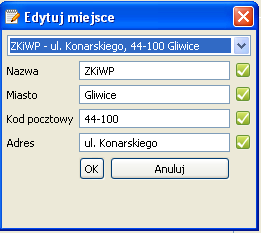
\includegraphics[width=0.45\textwidth]{images/editPlaceW}}    
  \hspace{2mm}
  \subfloat[Linux]{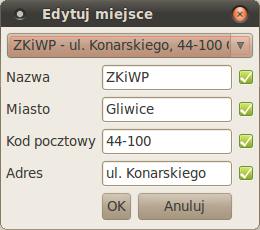
\includegraphics[width=0.45\textwidth]{images/editPlaceL}}
\caption{Okno edycji miejsc} 	
\label{editPlace}
\end{figure}

\begin{figure}[!htb]
\centering 		
  \subfloat[Windows]{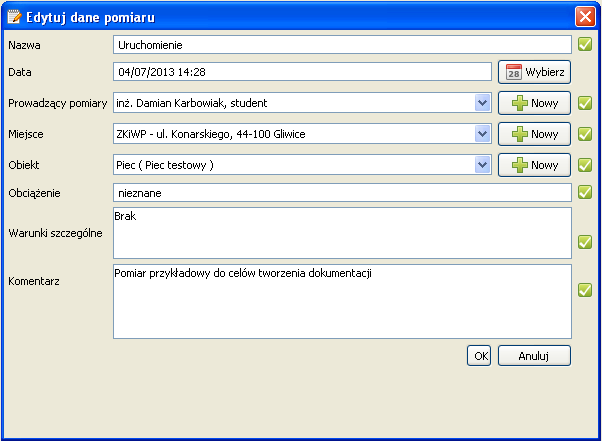
\includegraphics[width=0.45\textwidth]{images/editSurveyW}}    
  \hspace{2mm}
  \subfloat[Linux]{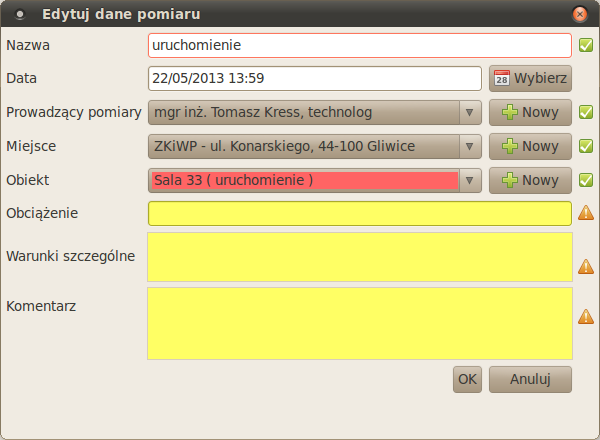
\includegraphics[width=0.45\textwidth]{images/editSurveyL}}
\caption{Okno edycji danych pomiaru} 	
\label{editSurvey}
\end{figure}

\begin{figure}[!htb]
\centering 		
  \subfloat[Windows]{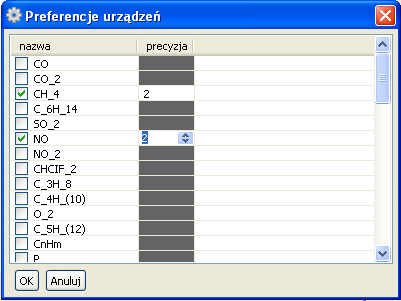
\includegraphics[width=0.45\textwidth]{images/editPrecisionW}}    
  \hspace{2mm}
  \subfloat[Linux]{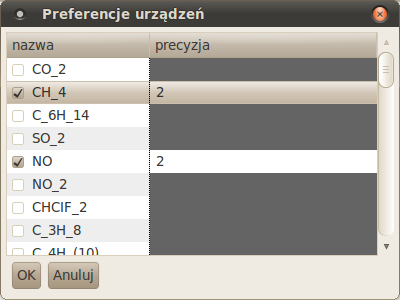
\includegraphics[width=0.45\textwidth]{images/editPrecisionL}}
\caption{Okno edycji precyzji pomiarowej} 	
\label{editPrecision}
\end{figure}

\begin{figure}[!htb]
\centering 		
  \subfloat[Windows]{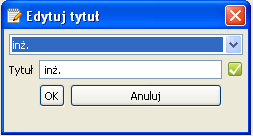
\includegraphics[width=0.45\textwidth]{images/editTitleW}}    
  \hspace{2mm}
  \subfloat[Linux]{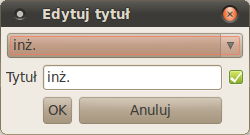
\includegraphics[width=0.45\textwidth]{images/editTitleL}}
\caption{Okno edycji tytułów naukowych} 	
\label{editTitle}
\end{figure}

\begin{figure}[!htb]
\centering 		
  \subfloat[Windows]{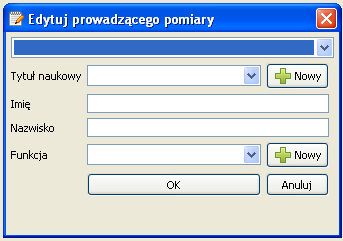
\includegraphics[width=0.45\textwidth]{images/editUserW}}    
  \hspace{2mm}
  \subfloat[Linux]{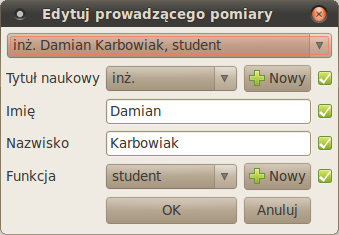
\includegraphics[width=0.45\textwidth]{images/editUserL}}
\caption{Okno edycji danych użytkownika} 	
\label{editUser}
\end{figure}

\begin{figure}[!htb]
\centering 		
  \subfloat[Windows]{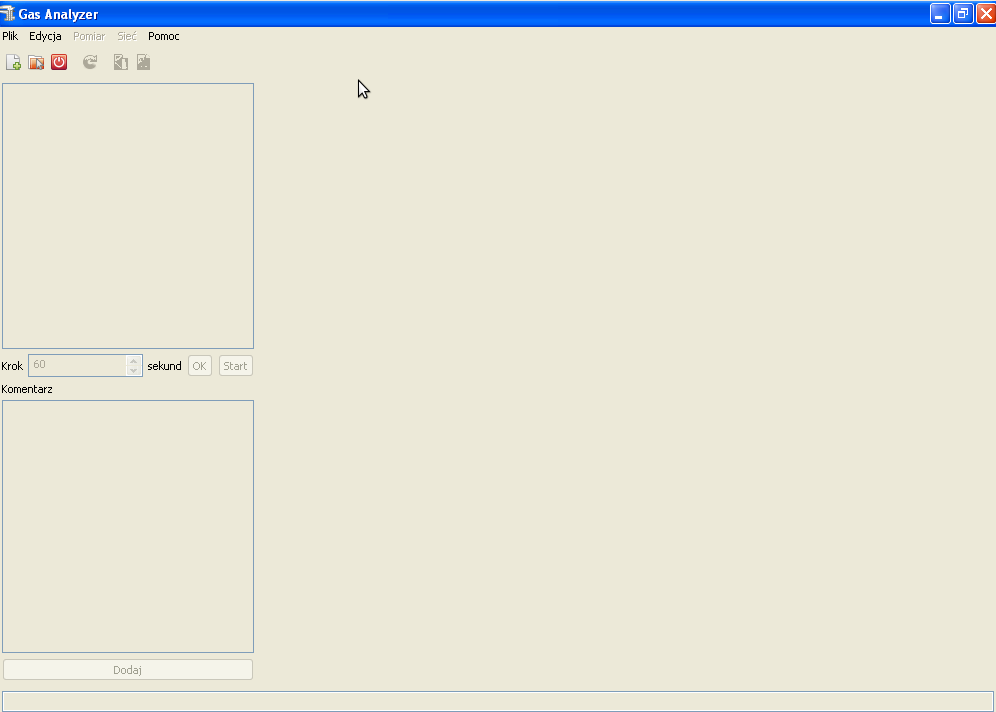
\includegraphics[width=0.45\textwidth]{images/mainW}}    
  \hspace{2mm}
  \subfloat[Linux]{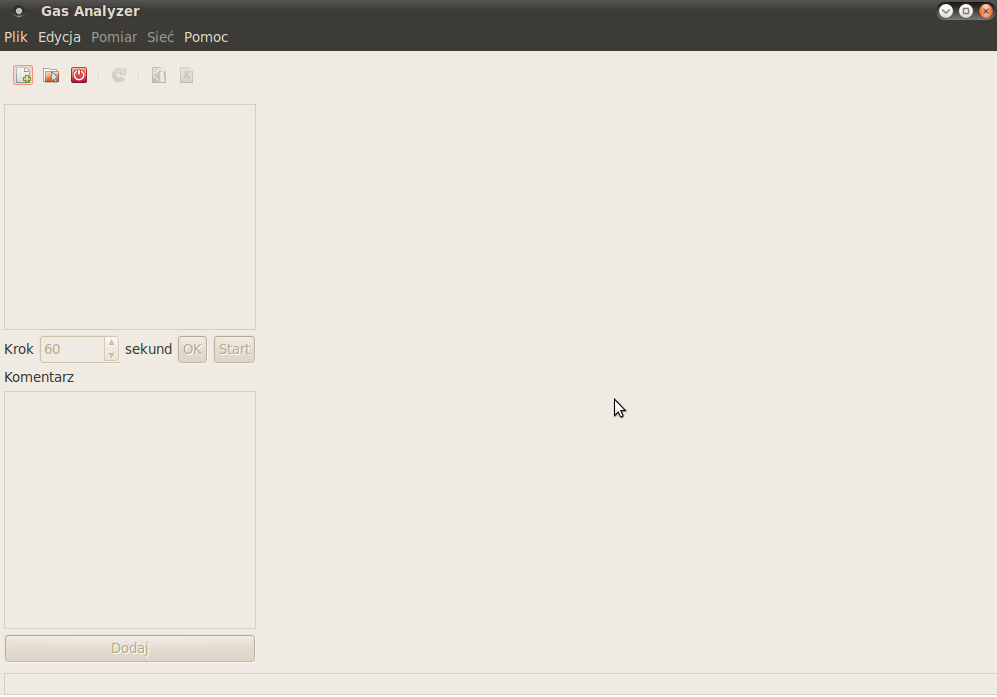
\includegraphics[width=0.45\textwidth]{images/mainL}}
\caption{Okno główne programu} 	
\label{main}
\end{figure}

\begin{figure}[!htb]
\centering 		
  \subfloat[Windows]{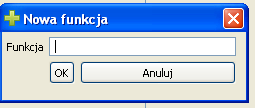
\includegraphics[width=0.45\textwidth]{images/newFunctionW}}    
  \hspace{2mm}
  \subfloat[Linux]{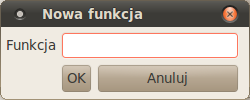
\includegraphics[width=0.45\textwidth]{images/newFunctionL}}
\caption{Okno dodawania funkcji} 	
\label{newFunction}
\end{figure}

\begin{figure}[!htb]
\centering 		
  \subfloat[Windows]{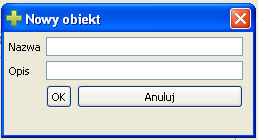
\includegraphics[width=0.45\textwidth]{images/newObjectW}}    
  \hspace{2mm}
  \subfloat[Linux]{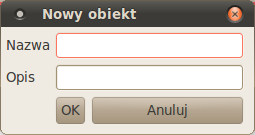
\includegraphics[width=0.45\textwidth]{images/newObjectL}}
\caption{Okno dodawania obiektu} 	
\label{newObject}
\end{figure}

\begin{figure}[!htb]
\centering 		
  \subfloat[Windows]{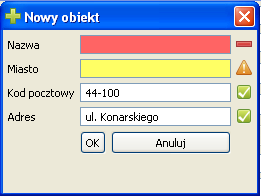
\includegraphics[width=0.45\textwidth]{images/newPlaceErrorW}}    
  \hspace{2mm}
  \subfloat[Linux]{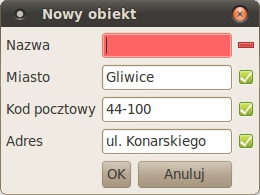
\includegraphics[width=0.45\textwidth]{images/newPlaceErrorL}}
\caption{Błąd przy dodawaniu nowego miejsca} 	
\label{newPlaceError}
\end{figure}

\begin{figure}[!htb]
\centering 		
  \subfloat[Windows]{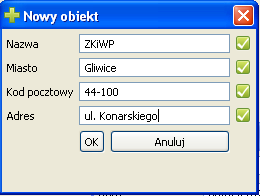
\includegraphics[width=0.45\textwidth]{images/newPlaceW}}    
  \hspace{2mm}
  \subfloat[Linux]{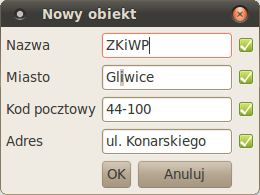
\includegraphics[width=0.45\textwidth]{images/newPlaceL}}
\caption{Okno dodawania miejsca} 	
\label{newPlace}
\end{figure}

\begin{figure}[!htb]
\centering 		
  \subfloat[Windows]{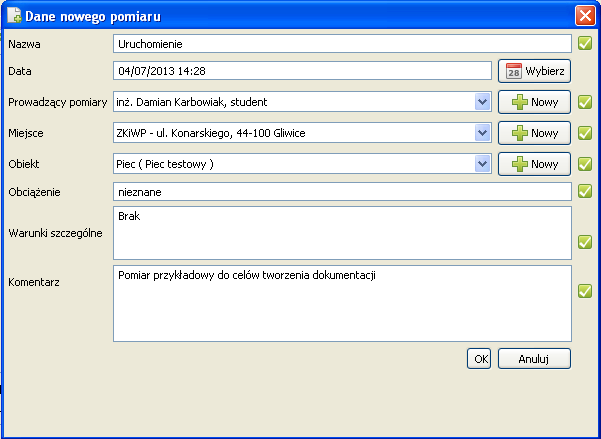
\includegraphics[width=0.45\textwidth]{images/newSurveyFilledW}}    
  \hspace{2mm}
  \subfloat[Linux]{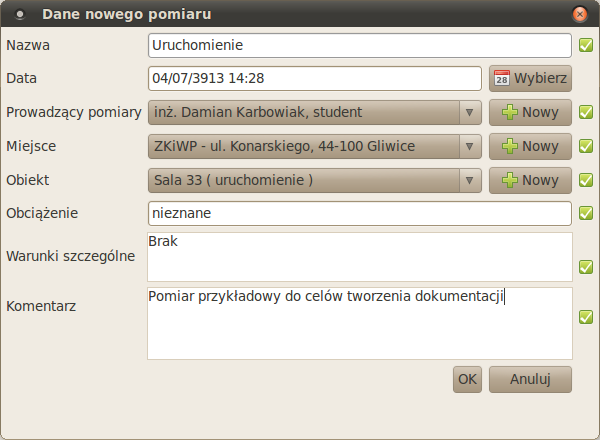
\includegraphics[width=0.45\textwidth]{images/newSurveyFilledL}}
\caption{Okno dodawania pomiaru po prawidłowym wypełnieniu} 	
\label{newSurveyFilled}
\end{figure}

\begin{figure}[!htb]
\centering 		
  \subfloat[Windows]{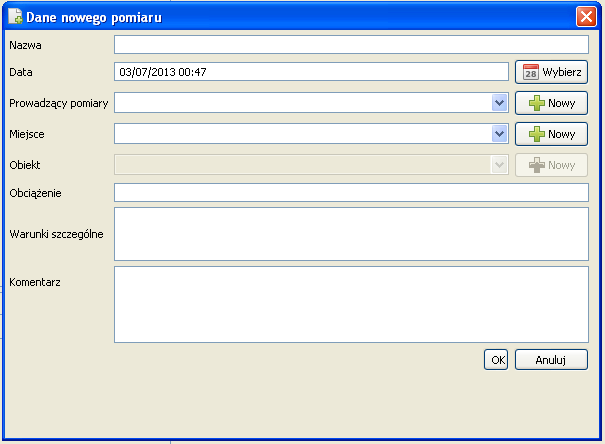
\includegraphics[width=0.45\textwidth]{images/newSurveyW}}    
  \hspace{2mm}
  \subfloat[Linux]{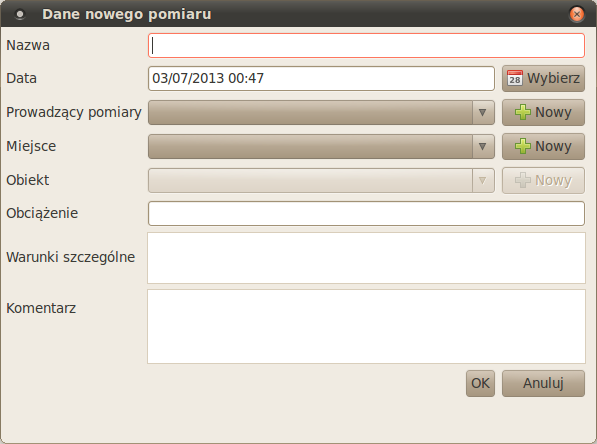
\includegraphics[width=0.45\textwidth]{images/newSurveyL}}
\caption{Okno dodawania pomiaru} 	
\label{newSurvey}
\end{figure}

\begin{figure}[!htb]
\centering 		
  \subfloat[Windows]{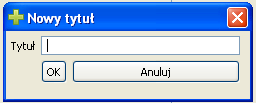
\includegraphics[width=0.45\textwidth]{images/newTitleW}}    
  \hspace{2mm}
  \subfloat[Linux]{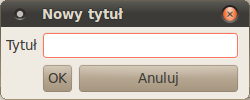
\includegraphics[width=0.45\textwidth]{images/newTitleL}}
\caption{Okno dodawania tytułu naukowego} 	
\label{newTitle}
\end{figure}

\begin{figure}[!htb]
\centering 		
  \subfloat[Windows]{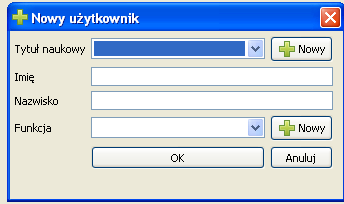
\includegraphics[width=0.45\textwidth]{images/newUserW}}    
  \hspace{2mm}
  \subfloat[Linux]{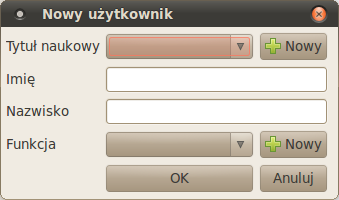
\includegraphics[width=0.45\textwidth]{images/newUserL}}
\caption{Okno dodawania użytkownika} 	
\label{newUser}
\end{figure}

\begin{figure}[!htb]
\centering 		
  \subfloat[Windows]{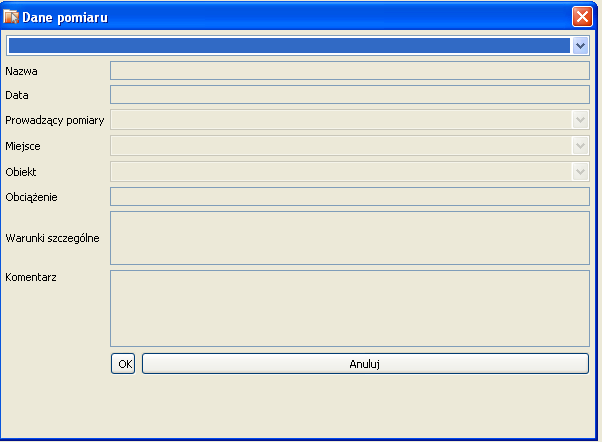
\includegraphics[width=0.45\textwidth]{images/openSurveyW}}    
  \hspace{2mm}
  \subfloat[Linux]{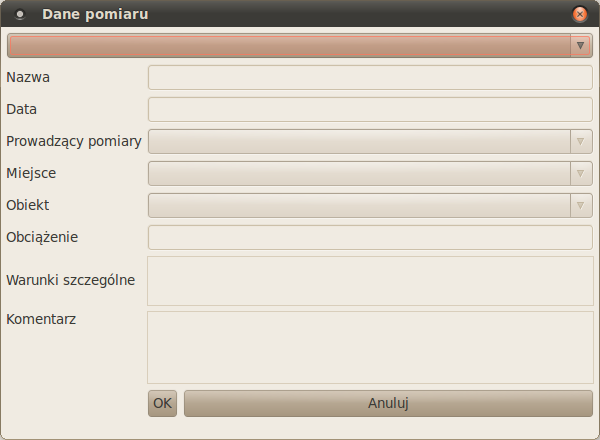
\includegraphics[width=0.45\textwidth]{images/openSurveyL}}
\caption{Okno otwierania pomiaru} 	
\label{openSurvey}
\end{figure}

\begin{figure}[!htb]
\centering 		
  \subfloat[Windows]{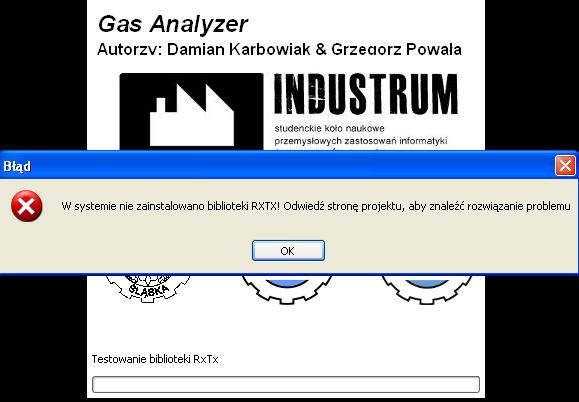
\includegraphics[width=0.45\textwidth]{images/rxtxErrorW}}    
  \hspace{2mm}
  \subfloat[Linux]{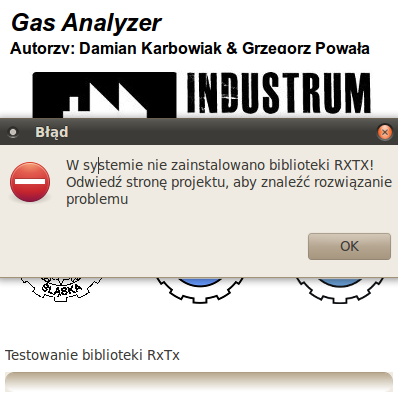
\includegraphics[width=0.45\textwidth]{images/rxtxErrorL}}
\caption{Okno błędu braku biblioteki RXTX} 	
\label{rxtxError}
\end{figure}

\begin{figure}[!htb]
\centering 		
  \subfloat[Windows]{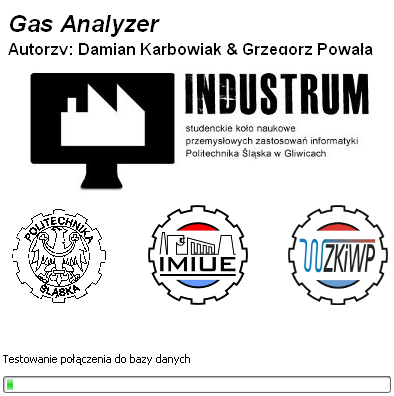
\includegraphics[width=0.45\textwidth]{images/splashScreenW}}    
  \hspace{2mm}
  \subfloat[Linux]{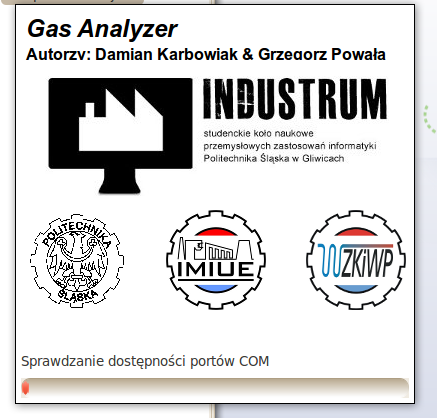
\includegraphics[width=0.45\textwidth]{images/splashScreenL}}
\caption{Okno ładowania aplikacji} 	
\label{splashScreen}
\end{figure}

\begin{figure}[!htb]
\centering 		
  \subfloat[Windows]{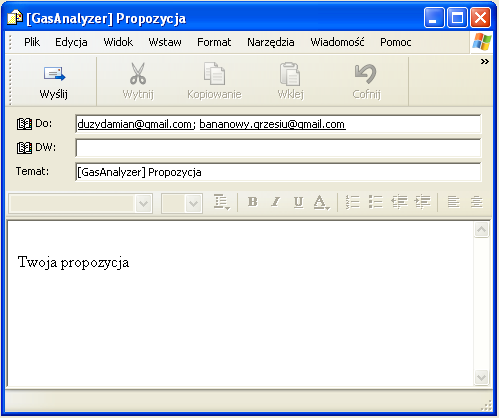
\includegraphics[width=0.45\textwidth]{images/suggestionW}}    
  \hspace{2mm}
  \subfloat[Linux]{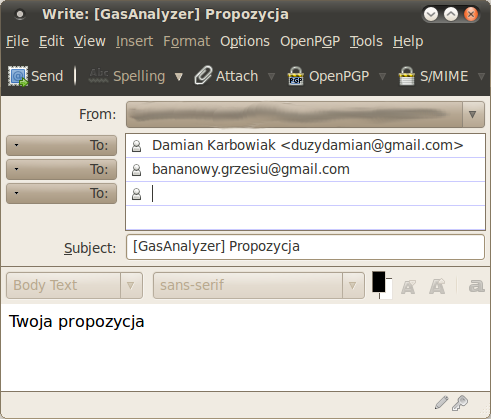
\includegraphics[width=0.45\textwidth]{images/suggestionL}}
\caption{Okno wysyłanie sugestii poprzez email} 	
\label{suggestion}
\end{figure}

\end{document}